\section{Arbeitsumgebung}

\subsection{Portainer[EK]}
\begin{figure}[H]
\centering
  
\includegraphics[scale=3]{images/protainer-logo.png}
  \caption{Protainer Logo (02.04.2020)}
  \url{https://pronto-core-cdn.prontomarketing.com/354/wp-content/uploads/sites/2/2018/07/logo-portainer-homepage.png}
\end{figure}
\subsubsection{Allgemein}
Bei portainer.io handelt es sich vereinfacht gesagt um ein Web-UI-Tool, welches ein grafisches Layer über Docker legt. Es handelt sich bei Portainer (Tool und Unternehmung teilen sich den Namen) um eine Open-Source Software, welche sich durch Supportdienstleistungen und spezielle Enterprise-Angebote finanziert.
\vspace{5mm}\par
Durch die GUI wird Zugriff auf die wichtigsten Funktionen von Docker bereitgestellt und bietet darüber hinaus nützliche Features, welche so nicht über die Docker-CLI verfügbar wären. Grundlegender Gedanke hinter so einer GUI ist es die möglichen Fehlerquellen, welche bei einer CLI-Nutzung zu Stande kommen, schnell erkennen zu können. Vor allem bei mehreren Containern kann so der Status durch ein Dashboard im Auge behalten werden, um systemkritische Elemente zeitnah erkennen zu können.
(vgl. \cite{Portainer})
\subsubsection{Entscheidungsprozess}
Von unserem Vorgesetzten der Firma MIC, wurde uns das Tool ans Herz gelegt, da es den Prozess der Problemfindung, durch klare visuelle Marker, in einem Multi-Container-Environment deutlich vereinfacht. 

\subsection{IntelliJ IDEA[EK]}
\begin{figure}[H]
\centering
  
\includegraphics[scale=0.1]{images/intellij_idea_logo.png}
  \caption{IntelliJ IDEA Logo (02.04.2020)}
  \url{https://upload.wikimedia.org/wikipedia/commons/thumb/d/d5/IntelliJ_IDEA_Logo.svg/1000px-IntelliJ_IDEA_Logo.svg.png}
\end{figure}
\subsubsection{Allgemein}
IntelliJ IDEA ist eine von JetBrains entwickelte IDE (zu Deutsch: Integrierte Entwicklungsumgebung). Im Jahre 2001 ins Lebens gerufen, steht IntelliJ heute in zwei Versionen zur Verfügung. Die kostenfreie Open-Source Community-Version wird unter der Apache-2.0 Lizenz vertrieben. Die kostenpflichtige Ultimate-Version wird als Shareware - Testmöglichkeit vor dem Kauf - vertrieben.
(vgl. \cite{IntelliJ-Background})
\subsubsection{Funktionsumfang}
Bei IntelliJ IDEA, handelt es sich um die JVM-IDE der IntelliJ Plattform, daher sind vor allem die JVM Sprachen Java, Scala, Groovy, Kotlin  und gegebenenfalls dazu verwendete Frameworks die Zielgruppe. Es werden aber auch andere Sprachen und Plattformen, wie zum Beispiel TypeScript und Android, unterstützt. Für diese Bereiche gibt es jedoch auch spezielle IDEs, welche auf IntelliJ IDEA basieren. Durch die Analyse des Codes, kann IntelliJ IDEA dem Entwickler Empfehlungen geben - die sogenannte Code-Completion. Die IDE unterstützt durch jenes Wissen den Nutzer bei dem fehleranfälligen Prozess des Refactorings. Neben der Unterstützung während des Schreibens des Codes sind auch Debugger- und Buildtools von Haus aus integriert. Die Erweiterbarkeit ist gegeben; sollten mehr, spezielle oder eigens entwickelte Funktionen benötigt werden, kann dies mittels Plugins gemacht werden.
(vgl. \cite{JetBrains-IDEA})
\subsubsection{Entscheidungsprozess}
Gründe für die Festlegung auf IntelliJ IDEA, war die Tatsache, dass die verwendete Programmiersprache Kotlin und das Build-Automation-Tool Gradle eine solide Integration in IntelliJ IDEA aufweisen. Nachvollziehbar, da die Sprache Kotlin selbst von JetBrains ins Leben gerufen wurden und Gradle ein essenzieller Teil der Kotlin-Idee ist - gezeigt auch dadurch, dass  die Möglichkeit besteht Kotlin-DSLs für die Build-Skripts zu verwenden. Darüber hinaus ist die persönliche Vertrautheit durch die intensive Verwendung dieser IDE in der HTL-Ausbildung durchaus groß, welche das Realisieren neuer Projekte in dieser deutlich fördert.

\subsection{Gradle[EK]}
\begin{figure}[H]
\centering
  
\includegraphics[scale=0.5]{images/gradle-logo.png}
  \caption{Gradle Logo (02.04.2020)}
  \url{https://gradle.org/images/gradle-knowledge-graph-logo.png?20170228}
\end{figure}
\subsubsection{Allgemein}
Gradle ist ein von Gradle Inc. entwickeltes Open-Source Build-Automation-Tool, welches im Jahre 2007 ins Leben gerufen wurde. Über Skripts werden die Build-Instruktionen angeben, diese können mithilfe von Groovy oder Kotlin DSLs geschrieben werden.
Vergleichbar ist Gradle mit Apache Ant und Apache Maven. Bei der Entwicklung von Gradle wurde versucht, die Flexibilität von Ant und das „Build-by-Convention“-Prinzip von Maven zusammenzuführen.
(vgl. \cite{Gradle-Background})
\subsubsection{Was ist ein Build-Automation-Tool?}
Ein Build-Automation-Tool beschreibt eine Anwendung, welche folgende Kriterien erfüllt: 
\vspace{1mm}\par
„Build-Automation ist der Prozess der Automatisierung der Erstellung eines Software-Builds und der damit verbundenen Prozesse, einschließlich dem Kompilieren von Computer-Quellcode in Binärcode, dem Packaging von Binärcode und dem Ausführen automatisierter Tests.“ \cite{Build-Automation}
\newpage
Einfach gesagt helfen Build-Tools dabei, folgende Beispiele zu automatisieren: 
\begin{itemize}
  \item Das Downloaden von Dependencies - Abhängigkeiten - von unserem Code, bei welchem wir zum Beispiel Libraries von Online-Respositories verwenden.
  \item Das Kompilieren vom Source-Code in für uns ausführbaren Code. Wir wollen zum Beispiel, anstatt selbst mit dem Compiler-Tool Kotlin-Code kompilieren zu müssen, diesen Prozess so automatisieren, dass mit einem Kopfdruck unser Code kompiliert und ausgeführt wird.
  \item Das Packaging so zu konfigurieren, dass wir am Ende den Code in der Form haben, welche wir weitergeben wollen. Ein Beispiel dafür wäre, dass wir unseren ganzen Kotlin-Code nach dem Build in einer großen JAR-Datei haben wollen.
  \item Das Ausführen von verschiedensten Tests, zu einem uns passenden Zeitpunkt. Wir wollen zum Beispiel, vor jedem Build sicher stellen, dass die gemachten Änderungen im Code auch noch immer die Kriterien der Unit-Tests erfüllen.
\end{itemize}
Zum Einsatz kommen Build-Tools dann, wenn ein manueller Build-Prozess durch die Anzahl an Dateien nicht mehr unter einem akzeptablen Zeitaufwand möglich ist. Ziel ist es, die Zeit des eigentlichen Entwickelns zu erhöhen.
(vgl. \cite{Gradle-Choice})
\newpage
\subsubsection{Entscheidungsprozess}
\begin{figure}[H]
\centering
  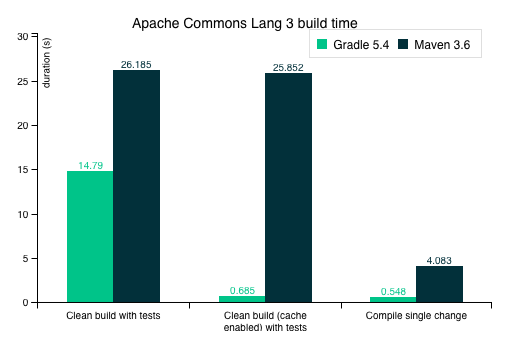
\includegraphics[scale=0.7]{images/gradle-vs-maven.png}
  \caption{Gradle vs. Maven (02.04.2020)}
  \url{https://gradle.org/maven-vs-gradle/}
\end{figure}
Die Entscheidung auf Gradle basiert auf dreierlei Argumenten: Flexibilität, Schnelligkeit und den Wissenserwerb. Die Flexibilität hat vor allem durch den modularen Ansatz dieser Arbeit einen großen Stellenwert. Aus der gezeigten Grafik können wir entnehmen, dass Gradle im Gegensatz zu seinem Pendant Maven beim Aspekt Schnelligkeit einen deutlichen Vorteil vorweist und damit wiederum Wartezeit in der Entwicklung erspart. Wissen in Gradle kann in vielen Softwareprojekten, vor allem größeren, von Nutzen sein - dieser Nutzen setzt jedoch ein bestimmtes Maß an Kenntnis mit diesem Tool voraus.

\subsection{Vim[EK]}
\begin{figure}[H]
\centering
  
\includegraphics[scale=0.2]{images/vim-logo.png}
  \caption{Vim Logo (02.04.2020)}
  \url{https://commons.wikimedia.org/wiki/File:Vimlogo.svg}
\end{figure}
\subsubsection{Allgemein}
Bei Vim handelt es sich sich um einen Command-Line-Editor, welcher mit den meisten Linux-Systemen, wie z.B. Ubuntu, bereits von Haus aus mitgeliefert wird. Ursprünge liegen schon in den 90er-Jahren, vor der Zeit der alltäglichen UI-Interfaces. Vim wird als eine sogenannte Charityware vertrieben, die Software an sich ist kostenfrei und Open-Source, jedoch wird der Nutzer ermutigt, für einen guten Zweck für Kinder in Uganda zu spenden, daher auch der Name Charityware.
(vgl. \cite{Vim-Background})
\subsubsection{Besonderheit}
Die Besonderheit von Vim liegt darin, dass die Idee der Bedienung darauf beruht, alle möglichen Dinge über Kommandos beziehungsweise Shortcuts zu lösen. Der Nachteil für neue Benutzer ergibt sich daraus, dass Vim anfangs überfordernd wirken kann. Dieser Nachteil ist aber auch der größte Vorteil, da sich eine Kenntnis dieser Funktionsweisen, schnell durch einen Geschwindigkeitsgewinn bemerkbar macht.
(vgl. \cite{Vim-Besonderheit})
\subsubsection{Entscheidungsprozess}
Da die verschiedenen Module auf den entsprechenden AWS-Instanzen laufen, fällt wie bei allen Server-Linux-Umgebungen die Möglichkeit einer Benutzung über die UI weg. So benötigt es einen Editor, welcher in dieser Umgebung nicht nur Text anzeigen kann, sondern dem Entwickler auch ein Syntax-Highlighting bietet. Durch Erfüllung dieser Kriterien wurde für Vim im Bereich der AWS-Instanzen zum Editor-of-Choice.

\newpage
\subsection{AWS[AA]}\label{ssec:aws}
\begin{figure}[H]
\centering
  
\includegraphics[scale=0.1]{images/aws-logo.png}
  \caption[AWS Logo (01.04.2020)]{AWS Logo (01.04.2020)}
  \label{fig:awslogo}
  \url{https://logos-download.com/wp-content/uploads/2016/12/Amazon_Web_Services_logo_AWS.png}
\end{figure}
Folgende Information wurden aus diesen Quellen herangezogen und überarbeitet.\\ (vgl. \cite{amazon_was_2020} \& \cite{amazon_ec2_2020})
\subsubsection{Allgemeine Beschreibung}
„Amazon Web Services (AWS) ist mit mehr als 175 Services, die umfangreiche Funktionen bieten und in global verteilten Rechenzentren bereitgestellt werden, die weltweit umfassendste und am häufigsten genutzte Cloud-Plattform. Millionen von Kunden – darunter einige der am schnellsten wachsenden Start-up-Unternehmen und der größten Konzerne sowie wichtige Behörden – vertrauen auf AWS, wenn es darum geht, agiler zu werden, Kosten zu senken und Innovationen schneller zu realisieren.“~\cite{amazon_was_2020}
\subsection{EC2}\label{ssec:ec2}
\subsubsection{Allgemeine Beschreibung}
„Amazon Elastic Compute Cloud (Amazon EC2) bietet eine skalierbare Rechenkapazität in der Amazon Web Services (AWS)-Cloud. Amazon EC2 beseitigt die Notwendigkeit, im Voraus in Hardware investieren zu müssen. Daher können Sie Anwendungen schneller entwickeln und bereitstellen. Sie können Amazon EC2 verwenden, um so viele oder so wenige virtuelle Server zu starten, wie Sie benötigen, Sicherheit und Netzwerk zu konfigurieren und den Speicher zu verwalten. Amazon EC2 können Sie auf- oder abwärts skalieren, um auf geänderte Anforderungen oder Datenverkehrsspitzen zu reagieren. Dies reduziert die Notwendigkeit, den Datenverkehr vorauszusagen.“ ~\cite{amazon_ec2_2020}
\newpage
\subsubsection{Funktionen von EC2}
\begin{itemize}
    \item Die primäre Funktion von EC2 sind Instanzen, die virtuelle Datenverarbeitungsumgebungen sind.
    \item Es speichert alle temporären Daten, die gelöscht werden in eigene Volumes, wenn ihre Instanz angehalten beziehungsweise beendet wird. Diese werden als Instanz Speicher Volume bezeichnet.
    \item Es werden bereits von EC2 vorkonfigurierte Vorlagen für Instanzen bereitgestellt. Diese heißen Amazon Machine Images (AMIs), die Komponenten für den Server verpacken können, oder auch Betriebssysteme und zusätzliche Software sein können.
    \item Es können auch Instanz Typen gesetzt werden. Diese beinhalten Konfigurationen für CPU, Arbeitsspeicher und Netzwerkkapazitäten.
    \item Die Anmeldung auf die AWS Maschinen erfolgt durch Schlüsselpaare. AWS selbst speichert den öffentlichen Schlüssel während der Benutzer den privaten Schlüssel speichern muss.
    \item EC2 hat Sicherheitsgruppen die für eine oder mehrere Instanzen benutzt werden können. In diesen wird festgehalten welche Protokolle, Ports und Quell IP Bereiche offen stehen und auf die Instanz zugreifen können.
\end{itemize}
\subsection{Warum AWS EC2?}
\subsubsection{Anforderung von MIC}
Die Anforderung war es die gesamte Systemarchitektur auf der Grundlage von AWS EC2 aufzubauen und dort skalierbar zu machen. Pro Schritt hätte es eine Instanz gegeben, um so mehrere Instanzen, des gleichen Prozesses, zu starten. Der ETL Prozess ist dadurch skalierbar und dynamischer.
\subsection{Probleme}
Durch die Sicherheitsgrundlagen des Unternehmens, war es immer nötig durch Port Forwarding die Ergebnisse der Funktionen an den nächsten Service weiterzuleiten. Denn jeder Port außer der achtziger Port war gesperrt. Deswegen war es immer notwendig, jede Funktion, die das Ergebnis an die nächste Instanz schickte über den achtziger Port gehen zu lassen.\\
Ein anderes Problem mit AWS war die Größe der Maschinen im EC2 Service. Durch die gewaltigen Daten die angekommen sind, war der Speicher der Instanzen oft voll und musste immer erweitert werden. 